\documentclass[a4paper, 12pt]{report}
\usepackage{times}

\usepackage[leftcaption]{sidecap}
\usepackage{subfigure} % figures can have sub chunks
\usepackage{geometry} % this maxes page usage, making the below unnecessary
\textwidth = 6.75in
\oddsidemargin = -0.25in
\textheight = 10in
\topmargin = -0.5in
\headheight = 15pt
\usepackage{fancyhdr}
\usepackage{pdfpages}

\pagestyle{fancy}
\lhead{{\it Alex Birch}}
\chead{ChibiPoint: Accessible Pointing for Web Applications}
\rhead{}
\lfoot{}
\cfoot{\thepage}
\rfoot{}

% for capitals font in signature
\usepackage[T1]{fontenc}

\usepackage{amsmath}

% For figures
\usepackage{graphicx}
\DeclareGraphicsExtensions{.pdf,.png,.jpg}
\usepackage{float}

\usepackage[sorting=none,backend=bibtex]{biblatex}
\bibliography{Diss}

\usepackage[colorlinks]{hyperref}
\usepackage{cleveref}
\crefformat{section}{section #2#1#3}
\crefdefaultlabelformat{[#2#1#3]}

\usepackage[nomain,acronym,toc,section,numberedsection=autolabel]{glossaries} % make a separate list of acronyms
%\makeindex
\makeglossaries

\title{ChibiPoint: Accessible Pointing for Web Applications}
\author{Alexander Birch}
\date{November 2013}
\begin{document}
\newglossaryentry{computer}
{
  name=computer,
  description={is a programmable machine that receives input,
               stores and manipulates data, and provides
               output in a useful format}
}


%\newacronym[\glsshortpluralkey=cas,\glslongpluralkey=contrived
%acronyms]{aca}{aca}{a contrived acronym}

\newacronym{rsi}{RSI}{Repetitive Strain Injury}
\newacronym{gui}{GUI}{Graphical User Interface}
\newacronym{w3c}{W3C}{World Wide Web Consortium}
\newacronym{wai}{WAI}{Web Accessibility Initiative}
\newacronym{wcag}{WCAG}{Web Content Accessibility Guidelines}
\newacronym{socog}{SOCOG}{The Sydney Organizing Committee for the Olympic Games}
\newacronym{cthdda}{Cth DDA}{Commonwealth Disability Discrimination Act 1992}
\newacronym{goms}{GOMS}{Goals, Operators, Methods, and Selection rules}

\newglossaryentry{accesskeys}
{
  name=access keys,
  description={a means for users to travel between distant or unrelated interface components using keyboard shortcuts}
}

\newglossaryentry{keybinding}
{
  name=key binding,
  plural=key bindings,
  description={mapping of keys, or combinations thereof, to actions}
}

\newglossaryentry{browserextension}
{
  name=web browser extension,
  description={(in the context of the Google Chrome web browser): extensions are small software programs that can modify and enhance the functionality of the Chrome browser. You write them using web technologies such as HTML, JavaScript, and CSS.}
}

\newglossaryentry{browsingcontext}
{
  name=browsing context,
  description={a window or tab in a web browser that hosts a webpage}
}
\maketitle
\tableofcontents
%\pagebreak

%\chapter*{Introduction}

\chapter{Introduction}

\section{Context and Motivation}
\section{Literature \& Technology Review}
% SUMMARY of literature review
\section{Problem statement and Hypothesis}
% Concise statement of problem
% State efficiency goal
\section{Goals and Methods}
% What we intend to solve, and how
\section{Results / Contributions}
% Summarise our most important findings
% Cast findings as contributions to research field
\section{Thesis overview}
% Overview of remainder of thesis

\chapter{Literature \& Technology Review}

\chapter{Requirements \& Design}

\chapter{Implementation}

\chapter{Evaluation}
\section{Overview}
The primary system comparison we sought to pursue was `ChibiPoint' versus `tabbing navigation'. We aimed also to evaluate the contribution made by the `flyouts' feature of ChibiPoint: whether it helps or hinders. As such, we evaluated three systems:
\begin{enumerate}
\item Tabbing navigation
\item ChibiPoint (with just the crosshairs feature enabled)
\item ChibiPoint (with both the crosshairs feature AND the flyouts feature enabled)
\end{enumerate}

We aimed to quantitatively evaluate the following things:
\begin{enumerate}
\item Which system is the most efficient for each class of navigation tested
\item Which system is the fastest for each class of navigation tested
\item Which system is preferred by the participants
\item Which system is considered by the participants to be easiest to use
\item How reasonable is the amount of keypressing demanded by each system, according to the participants
\end{enumerate}

Qualitative data was useful also, as it offered feedback on specific advantages or disadvantages of each system, as well as providing insight to usability and the reasons for user preferences.

We performed first a usability study, as a precursor to the more detailed quantitative testing. The usability study was expected to reveal how a new user approaches the system --- what level of instruction is necessary, and what problems are encountered with usage. Addressing issues here would reduce problems in the larger, quantitative study that followed.

Regarding the quantitative study: a pilot study was conducted first, to ensure that the study approach was effective, before widening the participation. Omissions from that pilot study were addressed.
A larger study then recruited 12 users to evaluate the systems in a counterbalanced $3 \times 8$ ANOVA (three systems, 8 navigation types).
% This would reveal which system was most suited to which kinds of pointing. Qualitative data was gathered also, to capture user preference.

\section{Study 1: Usability Study}
\section{Study 2: Quantitative Comparison of Pointing Systems}
\subsection{Outline}
A pilot study set the sequence for the full study to follow. The main output of the study was the evaluation of pointing systems; participants were instructed to complete several tasks of the following ilk:
\begin{enumerate}
\item Go to a specified website.
\item Using the specified pointing system, click a specified button/page element.
\end{enumerate}
After completing this set of tasks with one pointing system, the participant was asked to repeat it with another of the pointing systems under test, until all three systems had been tested. We counterbalanced the order in which pointing systems were allocated to participants, to reduce biases in learning the tasks or systems.

In addition to this evaluation of system performance, participants were asked to fill out two questionnaires. The first questionnaire was posed before the pointing tasks: participants declared their proficiencies with the computing concepts involved, as well as describing their demographic. The second questionnaire was posed after the pointing tasks, and asked the participants to give subjective feedback on the systems they used.

\subsection{Demographic}
All participants were known personally by the researcher, with a majority (9) explicitly identifying as being current Computer Science students.

The mean average age for participants was 22.58, with a standard deviation of 2.151. The range was 21--28. These data are tabulated in Figure \ref{fig:partic_age}.
A quarter of participants were female, the rest were male (Figure \ref{fig:partic_gender}).

\subsubsection{Proficiencies}
Most participants were frequent users of computing devices; 5 using computers or smartphones for 13+ hours per day, 5 using the same for 7-9 hours, and just 2 using devices for 4-6 hours. Other categories (0-1, 2-3, 10-12) were offered, but no participants identified with these. These frequencies can be seen in Figure \ref{fig:partic_computerHours}.

Many participants (5) preferred to navigate using a mouse, with a majority (6) recruiting hotkeys in addition to the mouse. Only one participant actually preferred keyboard controls, and no participant identified with completely requiring full mouse support or full keyboard support (Figure \ref{fig:partic_proficiency}).

Touch-typing proficiency was rated on a five-point scale ranging from the sentiment `I look at every key before pressing' to `I always type without even a reference glance at the keyboard' (Figure \ref{fig:partic_ttype}. Participants on (mean) average considered themselves a 3.42. A standard deviation of 1.084 was observed. Two primary users of the Dvorak keyboard layout were asked to use the (familiar, but not preferred) Qwerty layout during this study, and rated their touch-typing with respect to the constraint that they would be typing in Qwerty during this time.

A majority (11) used mainly Windows as their desktop Operating System. Browser choice was more divided, with 7 participants using mainly Google Chrome, 3 Firefox and 1 `Other' (at the time disclosed to be Safari, which was not an option offered on the questionnaire).

\subsubsection{Disability}
Regarding participant's exposure to accessibility needs or solutions, three had used Dragon NaturallySpeaking speech-to-text. The two who elaborated on the extent of their use of speech-to-text described only limited use. No participant had --- at the time, or ever --- had computer-relevant vision difficulties. Two had had in the past minor experiences with RSI, with one describing ``RSI from mouse use, but nothing too severe to require a large change in typing/clicking'', the other elaborating ``Have changed input device due to pain in very specific circumstances.''. No participants had RSI at the time of the study.

\subsection{Methodology}
The following describes the methodology for the full study. Deviations exclusive to the pilot study are disclosed in its separate section.

The researcher followed a script to ensure that all instances of the study were performed the same way.

Participants were briefed on the purpose of the dissertation and of the study, as well as what participation in the study would entail. They were assured that no identifying information would be kept about them, that it was the system performance being measured rather than their personal performance, and that they were free to withdraw participation at any point. With these explained, participants were asked to sign a permission slip, and were offered also a copy in case they wished to contact the researchers after the fact.

Participants were assigned a unique number. This enabled both the questionnaires they would fill in to be related as being from the same participant. Additionally participants were assigned a sequence in which to evaluate the three systems. Biases pertaining to the order in which systems are used, were counterbalanced by testing using all sequence permutations of the three systems equally. There were 6 permutations, so the study recruited a multiple of this: 12 participants.

The study began with the first questionnaire's being allocated. This asked participants to disclose their demographic (occupation, gender and age).

The participants began the testing activity by reading instructions on the system they had been allocated. The researcher then guided them through a training scenario to confirm that they had understood the instructions. During this training period, the researcher would answer any questions and correct any mistakes that occurred. In the case of learning the system `ChibiPoint with crosshairs AND flyouts' before learning the system `ChibiPoint with crosshairs ONLY', participants were trained in the use of both features in turn.

[INCOMPLETE]

\subsection{Metrics}
The metric that was most important to study was efficiency --- how many keypresses (and by extension, how much exertion) are required for a given navigation task. Secondary to this metric was time taken by each system to perform a navigation task --- it is preferred, but not essential, for the system to be fast; the main priority is reducing exertion, which is connected to efficiency.

During the navigation tasks, user keypresses were recorded, as well as the times that they occurred. We recorded only keypresses relevant to pointing with the current system. For example, attempts to use the `tab' key during use of ChibiPoint were intercepted, and answered with an alert to the user that tabbing was disallowed. We disregarded keyboard input that did not invoke functionality within tabbing or the currently activated version of ChibiPoint. Page scrolling via the keyboard was considered unrelated to pointing, and so was not recorded. Attempts to invoke flyouts were only recorded when said flyout was present; if no flyouts were created (for example because no clickables are in the specified area, or if flyouts are disabled altogether), then the keypress was disregarded.

The post-task questionnaire asked participants to give subjective feedback on the systems they used. Some of the feedback was quantitative --- which was the preferred pointing system, how easy was each system to use, and how reasonable was the amount of key pressing required --- and some of the feedback was qualitative, asking for general thoughts on the task and systems.

\subsection{Pilot Study}

\chapter{Results}

\chapter{Conclusions \& Future work}

\chapter{Figures}
%[trim=0.0cm 11cm 0.0cm 11cm,clip]
%[viewport=0 0 390 610,clip,width=8in]
%[viewport=0 0 11cm 5cm,clip]
%fbox
\begin{figure}[ht]
\centerline{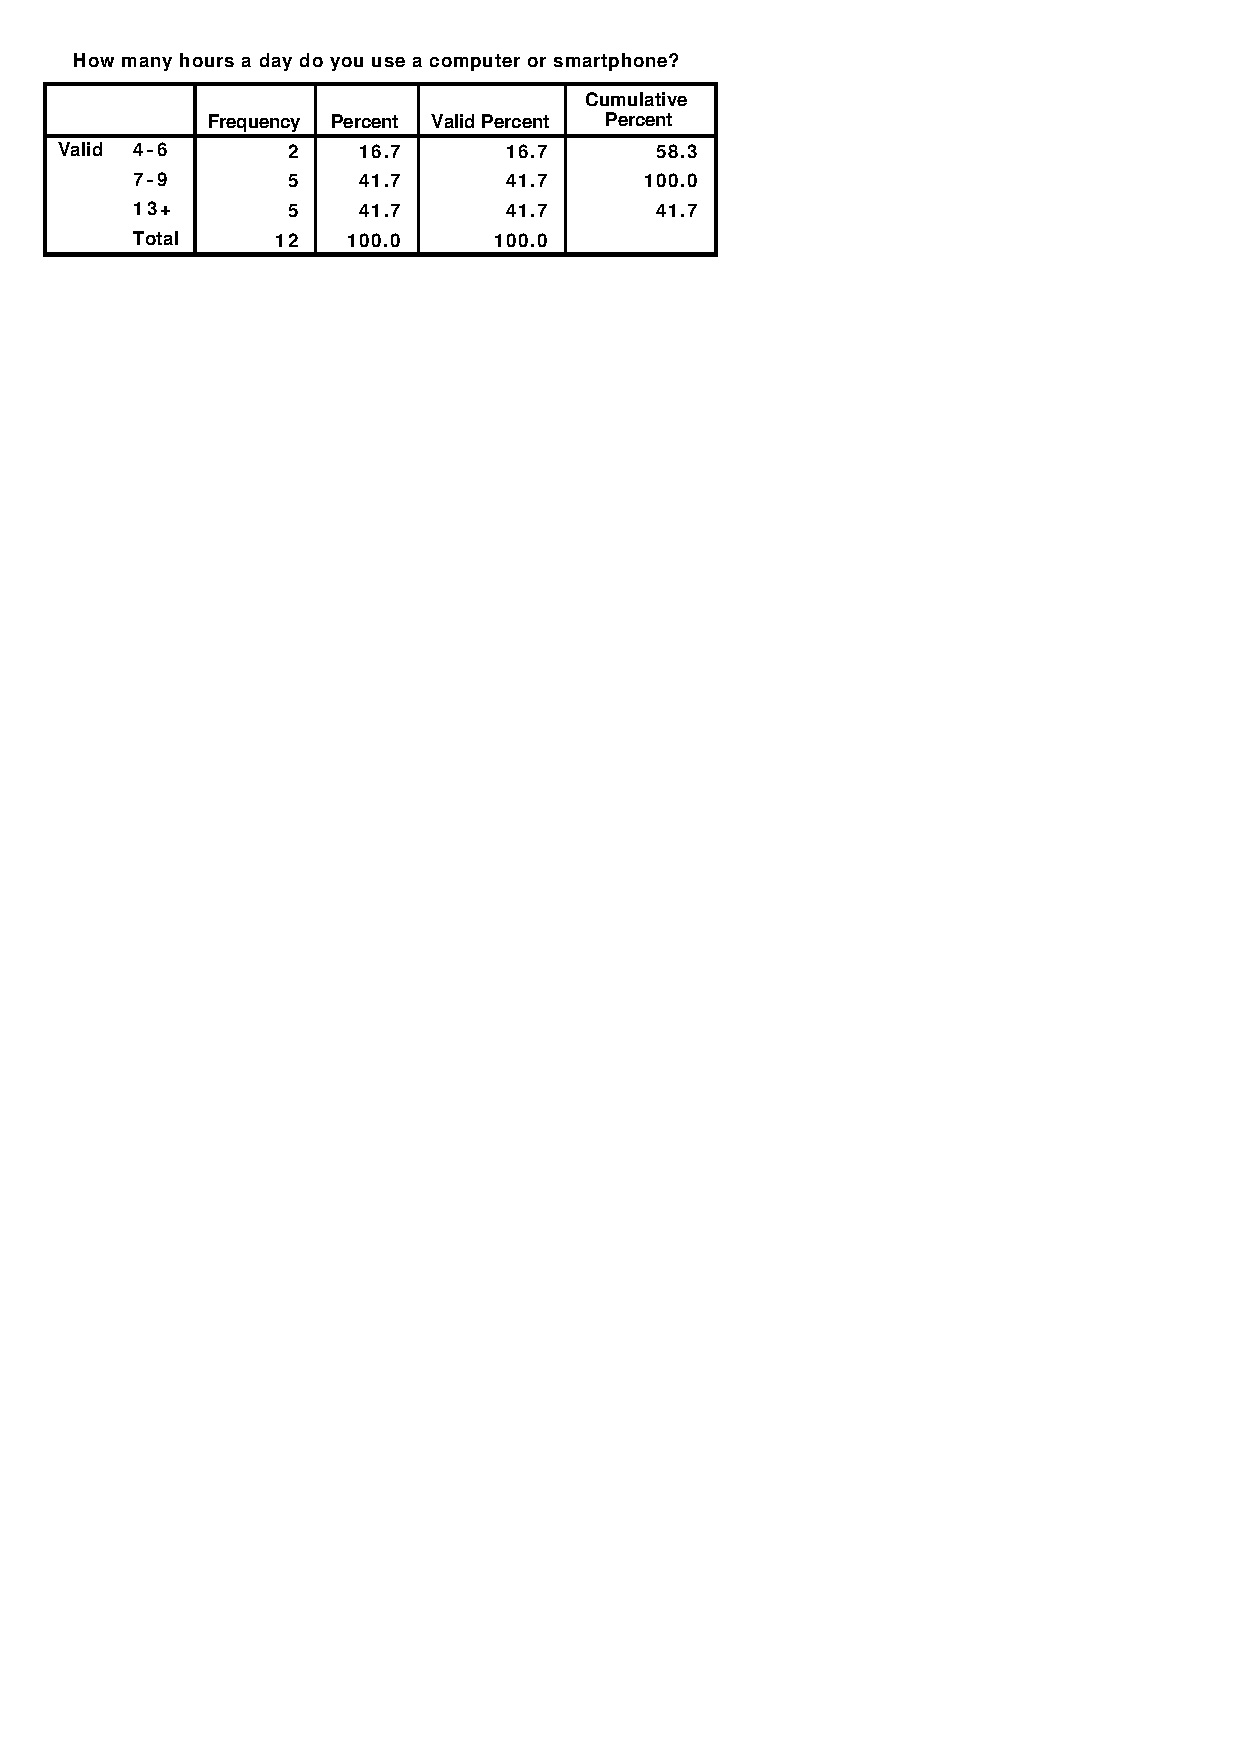
\includegraphics{figures/ComputerHours.pdf}}
\caption{Device usage by participant}
\label{fig:partic_computerHours}
\end{figure}

\begin{figure}[ht]
\centerline{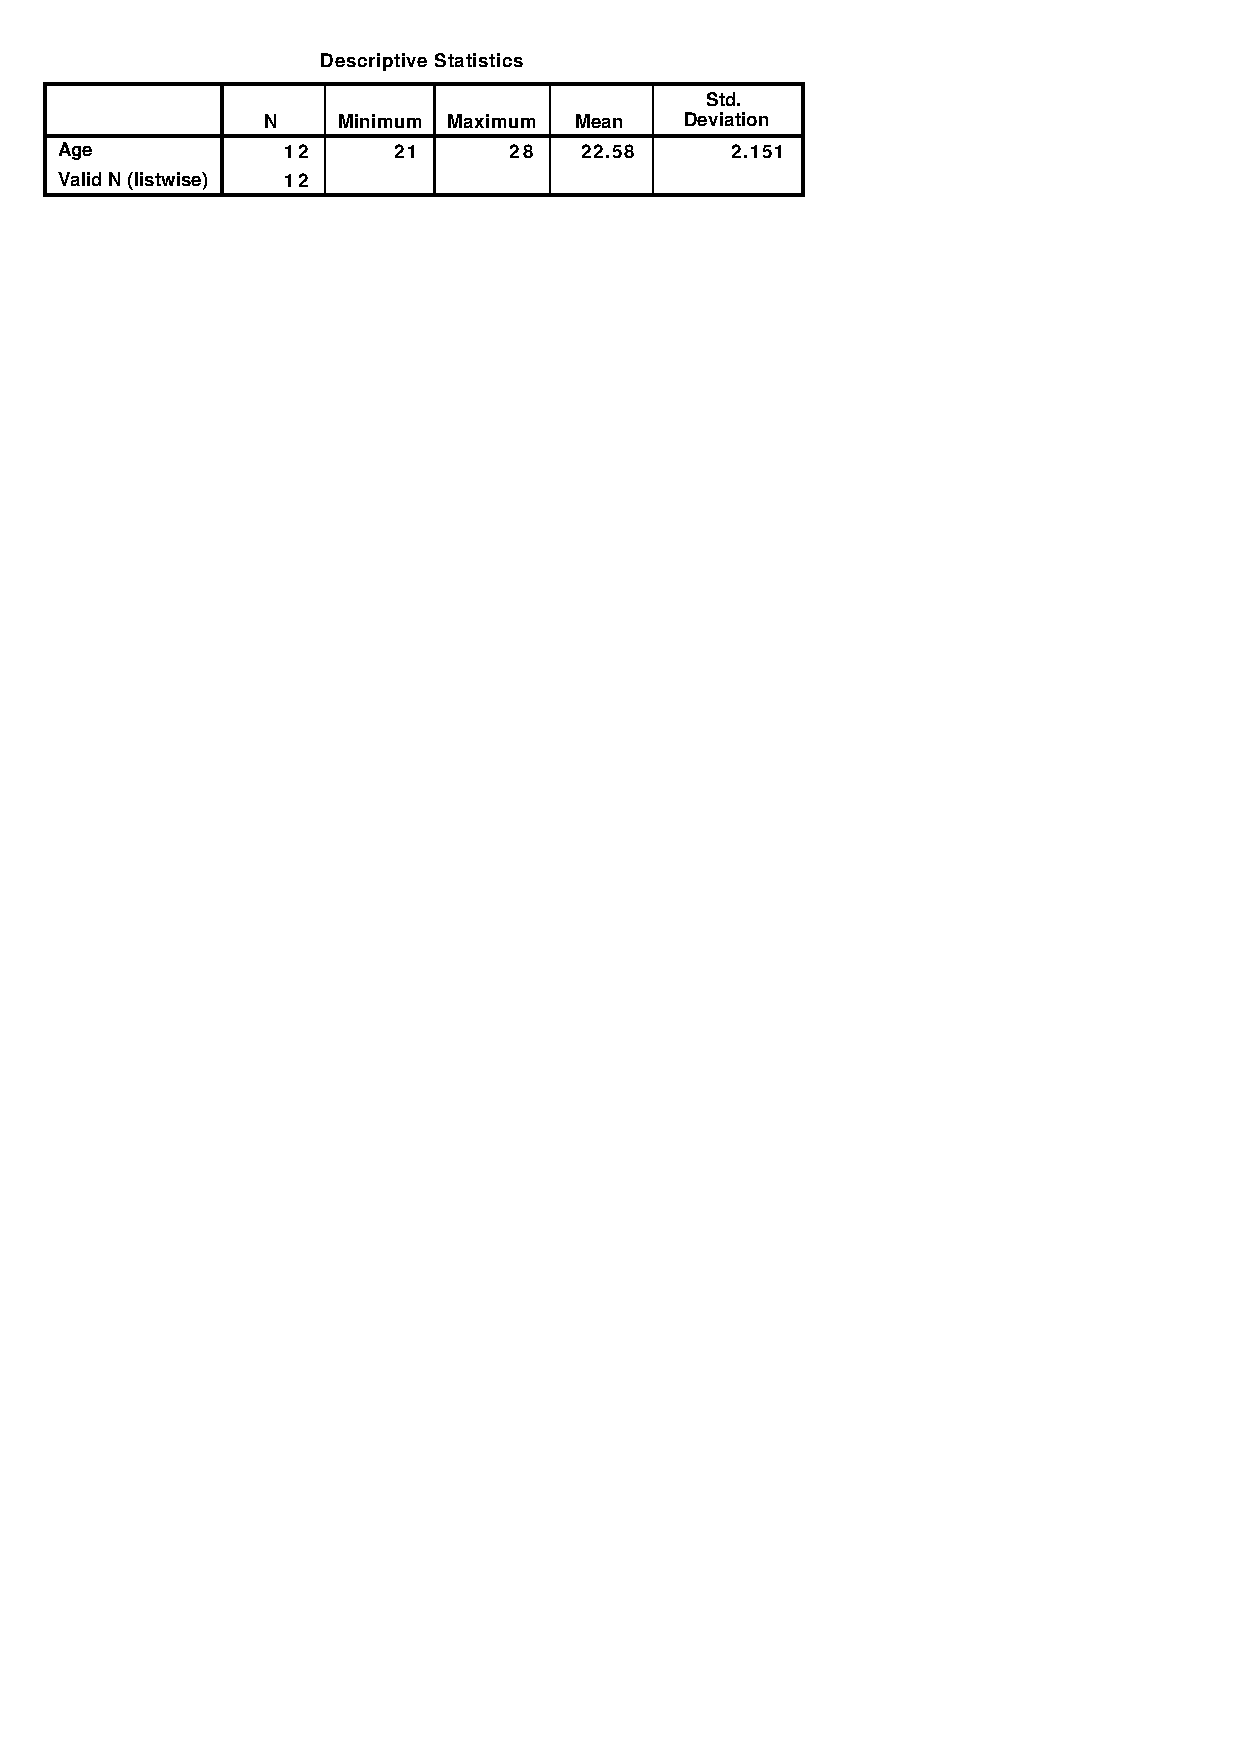
\includegraphics{figures/Age.pdf}}
\caption{Age of participant}
\label{fig:partic_age}
\end{figure}

\begin{figure}[ht]
\centerline{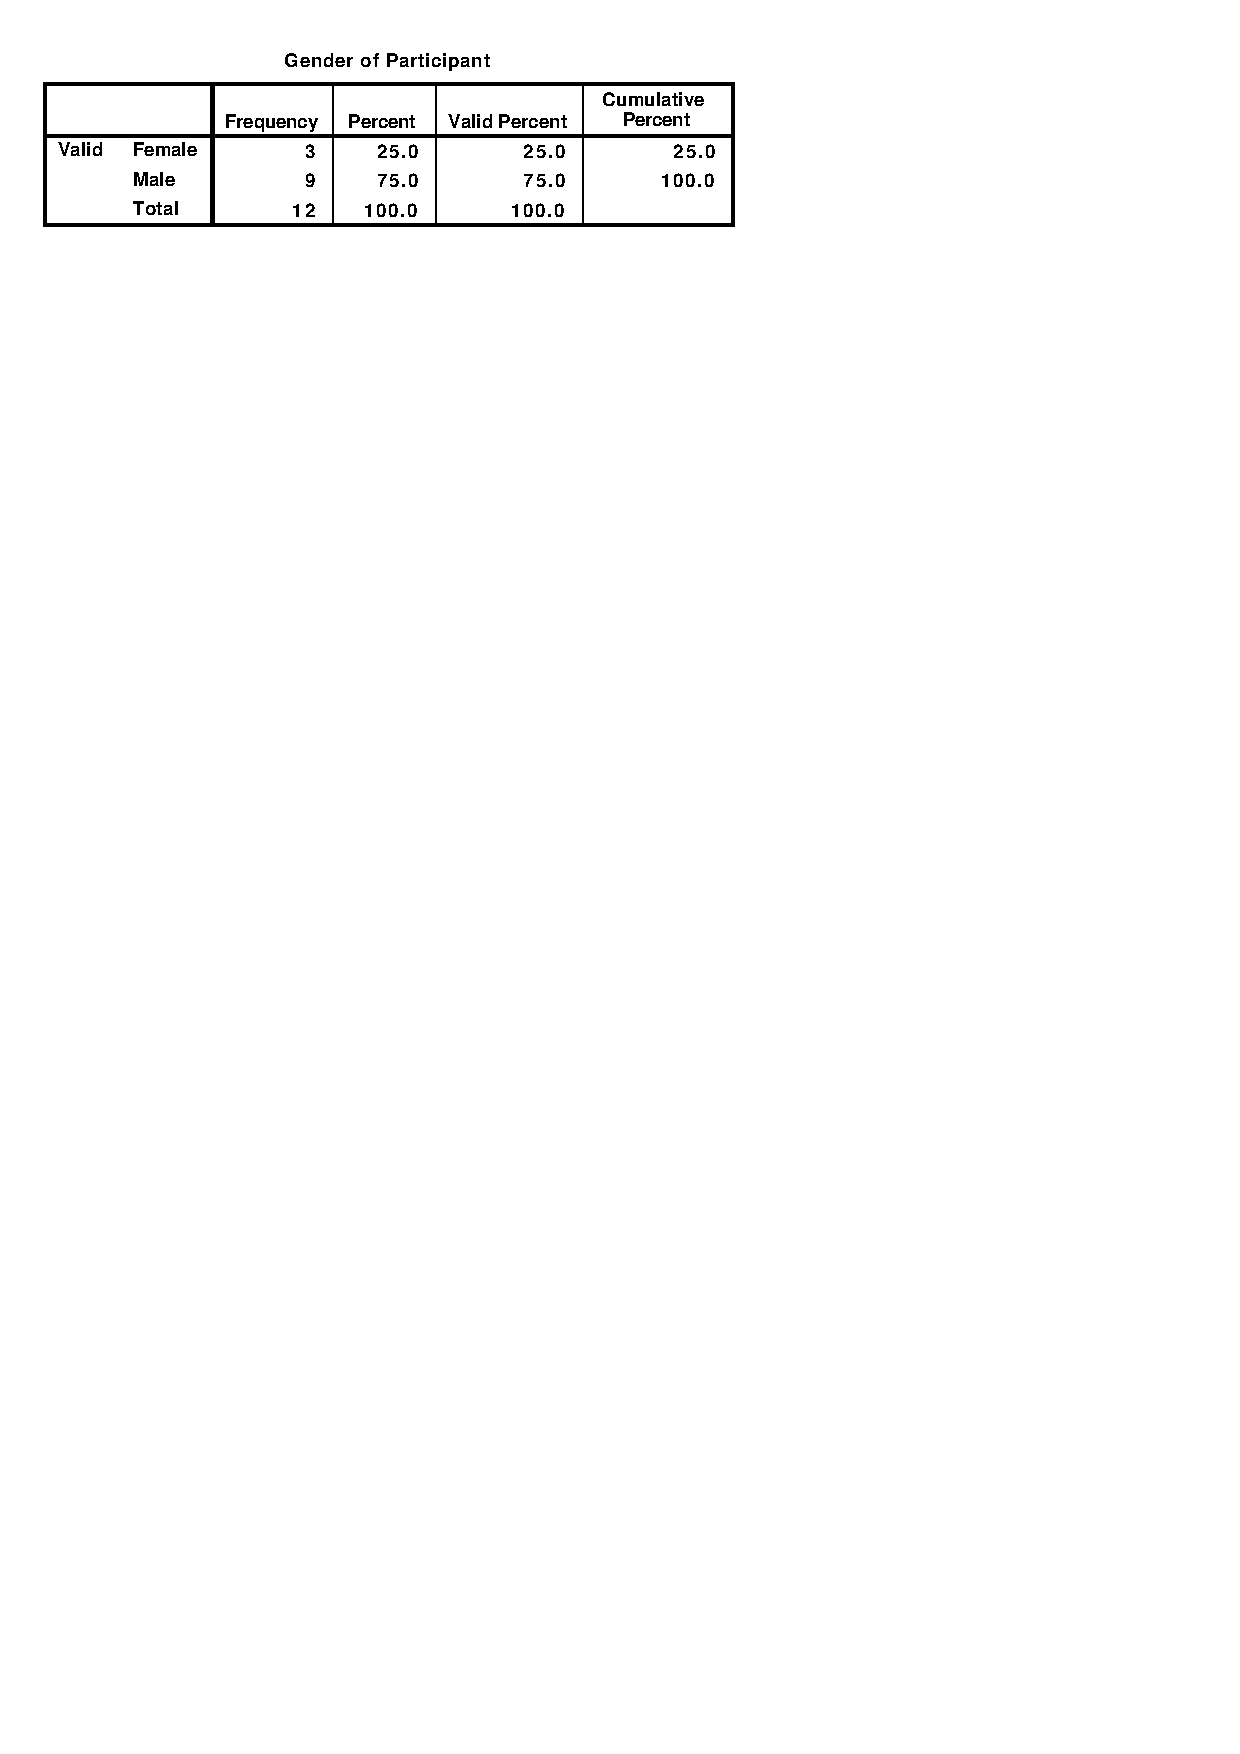
\includegraphics{figures/Gender.pdf}}
\caption{Gender of participant}
\label{fig:partic_gender}
\end{figure}

\begin{figure}[ht]
\centerline{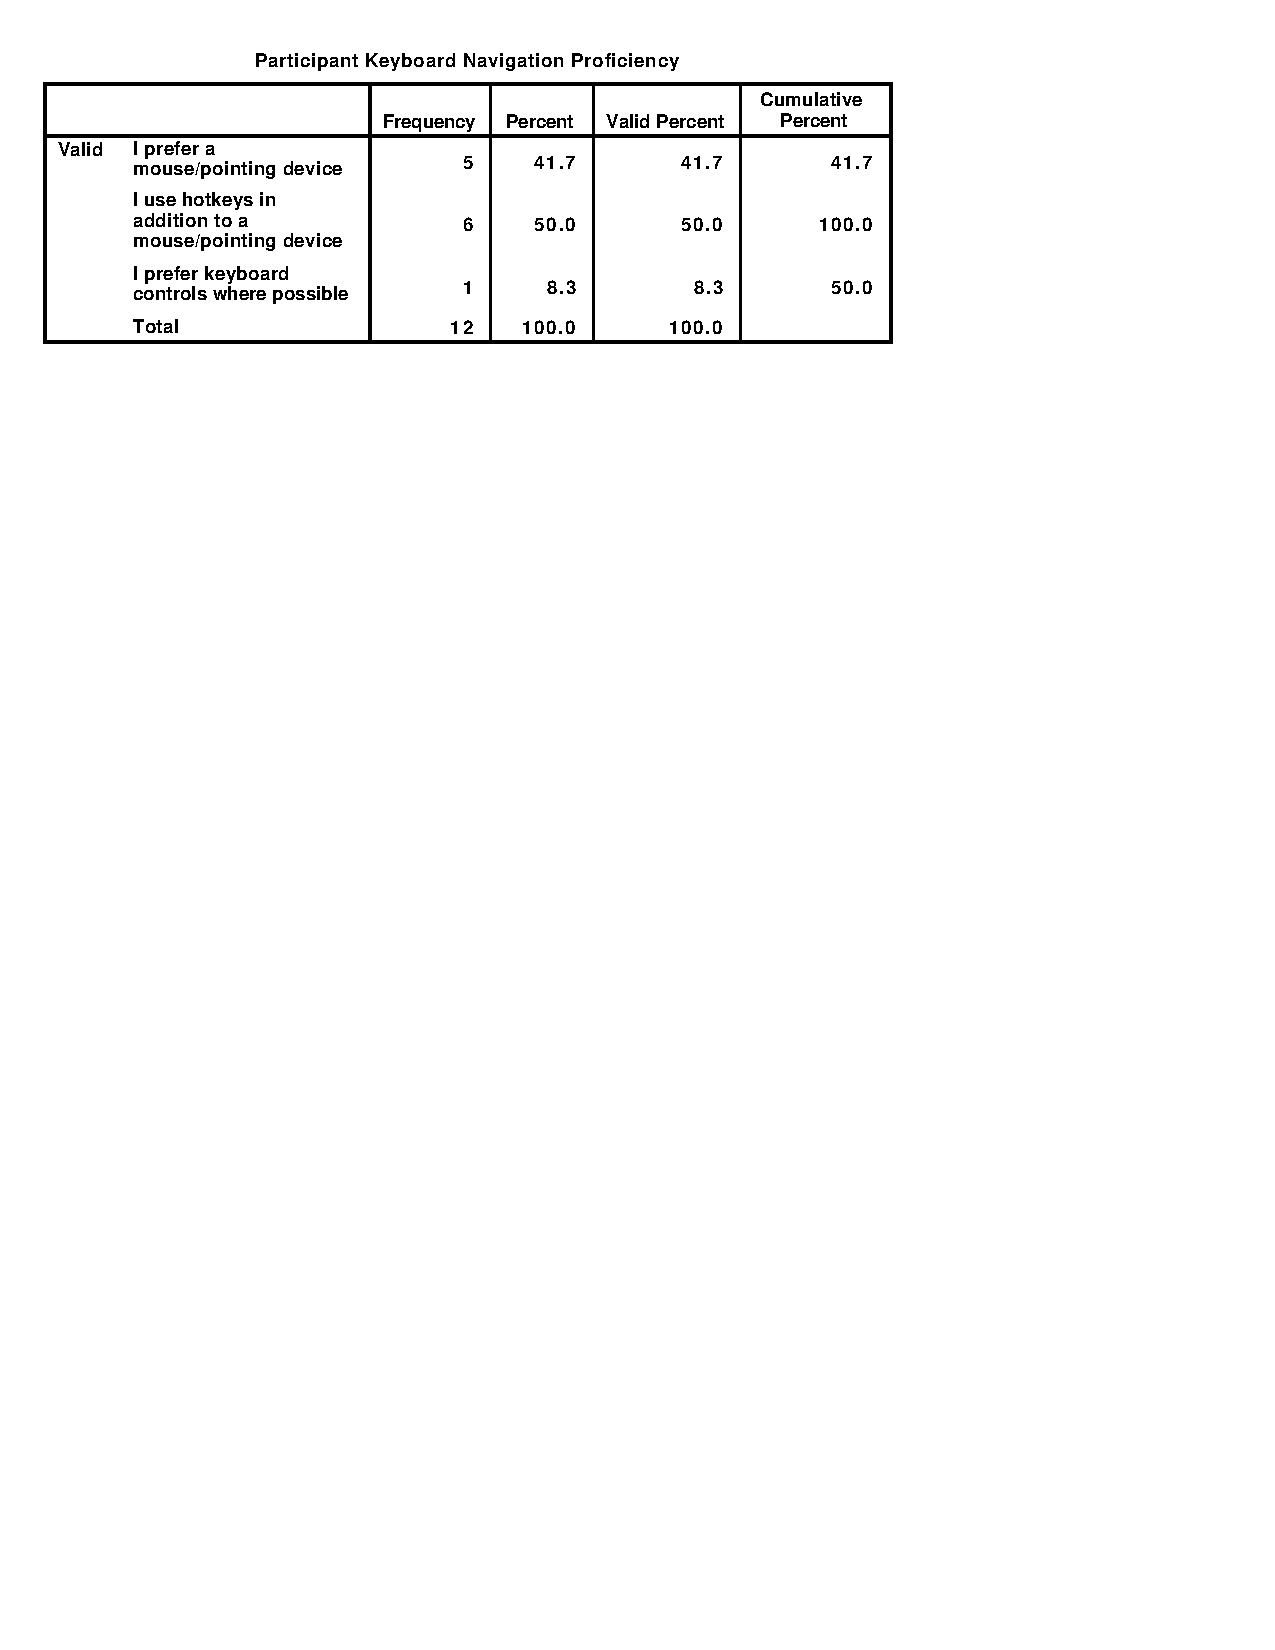
\includegraphics{figures/Proficiency.pdf}}
\caption{Keyboard Navigation Proficiency of Participants}
\label{fig:partic_proficiency}
\medskip
\small
Participants were asked to pick which of these sentiments they identified best with. The statements attempted to describe a proficiency scale for keyboard usage:
\begin{enumerate}
\item I need a mouse/pointing device
\item I prefer a mouse/pointing device
\item I use hotkeys in addition to a mouse/pointing device
\item I prefer keyboard controls where possible
\item I strongly prefer full keyboard support
\end{enumerate}
Votes were cast only for the middle descriptors, 2--4.
\end{figure}

\begin{figure}[ht]
\centerline{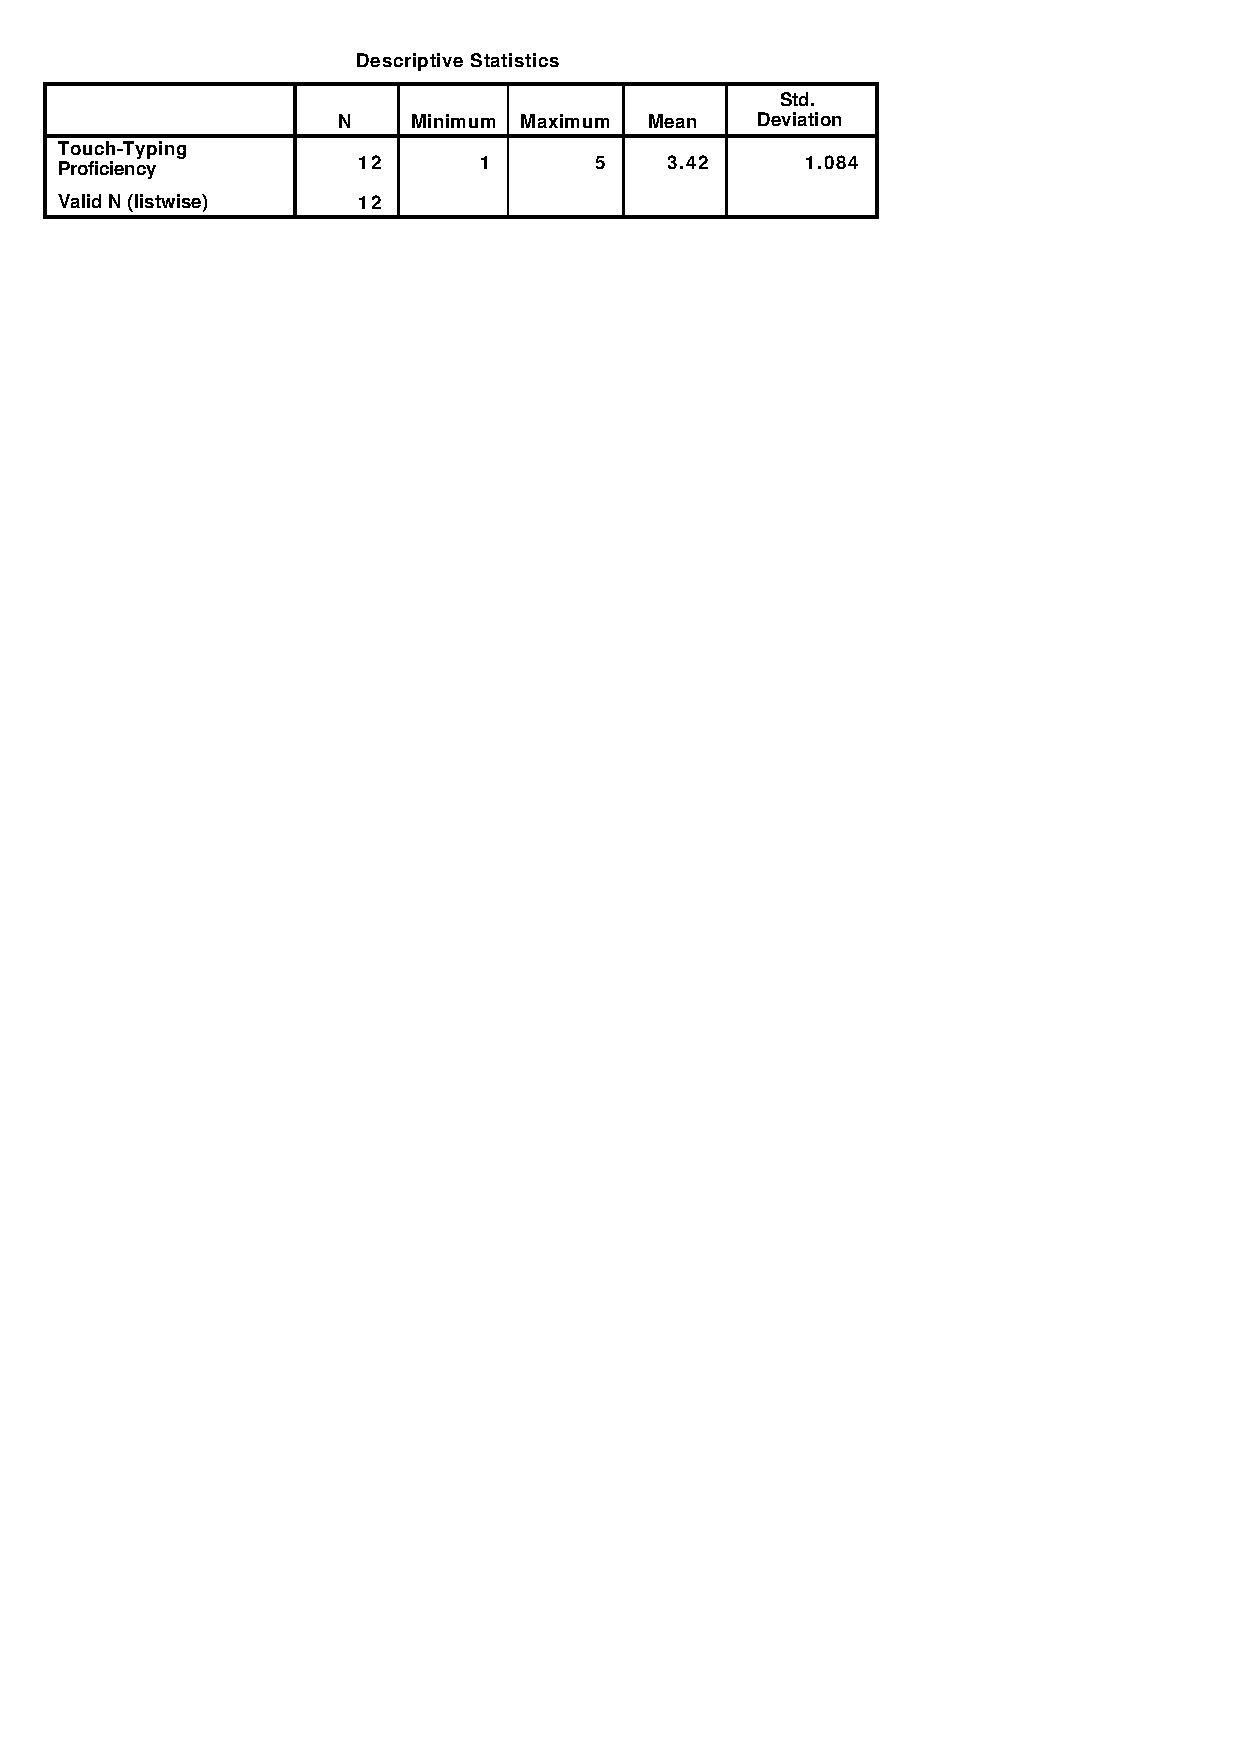
\includegraphics{figures/TouchTyping.pdf}}
\caption{Touch-Typing Proficiency of Participants}
\label{fig:partic_ttype}
\medskip
\small
Touch-typing proficiency was rated on a five-point scale ranging from the sentiment `I look at every key before pressing' to `I always type without even a reference glance at the keyboard'.
\end{figure}


\pagebreak
\printglossary[title=Terms]

%\nocite{*}
%\nocite{Doe:2009:Online}
\pagebreak
\printbibliography

\pagebreak
\chapter{Appendices}

\end{document}